\documentclass[../tesis_main.tex]{subfiles}


\chapter{Resultados y conclusiones}
En esta sección analizaremos los resultados obtenidos al probar el algoritmo RANSAC para encontrar planos modificando el numero de iteraciones. Observaremos el comportamiento del error y el tiempo de ejecución a fin de encontrar el número óptimo de iteraciones para este algoritmo.\\

	El proceso para el análisis de datos fue el siguiente: se propuso un modelo de plano conocido por el usuario. Dicho modelo se obtuvo a partir del conocimiento de la altura del plano en este caso una mesa. Posteriormente se cuantificó la cantidad de puntos que entraban en este modelo ideal y se tomó como base para la medición de errores. Continuando con el procedimiento se modificó el algoritmo para realizar un número determinado de iteraciones (600, 200, 100, 50, 30, 24 y 20) y se midió el error relativo y el tiempo de ejecución, en cada uno de estos procedimientos.\\

	Para probar el algoritmo con 600 iteraciones se tomaron 50 muestras los resultados se pueden observar en la siguiente gráfica.\\


	\begin{figure}[H]
		\begin{center}
		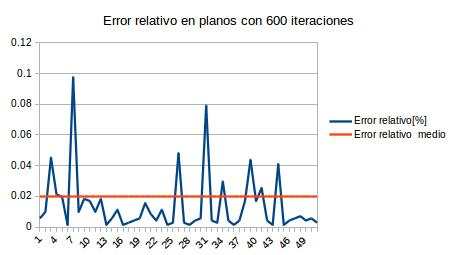
\includegraphics[width=10.5cm, height=3.4cm]{resultados/600_errRel.jpg}	
		\caption{Gráfica correspondiente al error relativo para el algoritmo RANSAC para detección de planos con 600 iteraciones.}

		\end{center}
	\end{figure}

	\begin{figure}[H]
		\begin{center}
		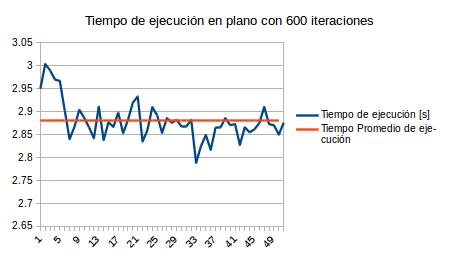
\includegraphics[width=12.5cm, height=6.0cm]{resultados/600_timeExec.jpg}
		\caption{Gráfica correspondiente al tiempo de ejecución para el algoritmo RANSAC para detección de planos con 600 iteraciones.}
		\end{center}
	\end{figure}

	Se tomaron 50 muestras para el algoritmo modificado con 200 iteraciones. los resultados se pueden observar en la siguiente gráfica.\\

	\begin{figure}[H]

		\begin{subfigure}[h]{.5\textwidth}
		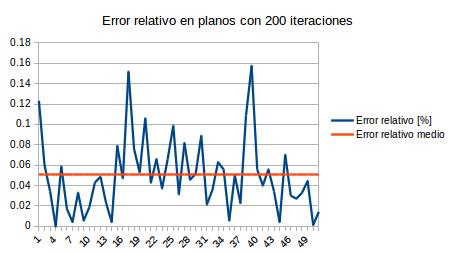
\includegraphics[width=8.5cm, height=5.0cm]{resultados/200_errRel.jpg}	
		\end{subfigure}%
		\begin{subfigure}[h]{.5\textwidth}
		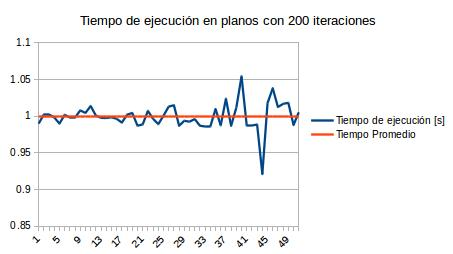
\includegraphics[width=8.5cm, height=5.0cm]{resultados/200_timeExec.jpg}
		\end{subfigure}
	
	\caption{Gráficas correspondientes al error relativo y tiempo de ejecución para el algoritmo RANSAC con 200 iteraciones.}

	\end{figure}

	Se continuó con el mismo principio para el algoritmo modificado con 100, 50, 30, 24 y 20 iteraciones respectivamente. Los resultados se pueden observar en las gráficas anexadas a continuación.\\


	\begin{figure}[H]

		\begin{subfigure}[h]{.5\textwidth}
		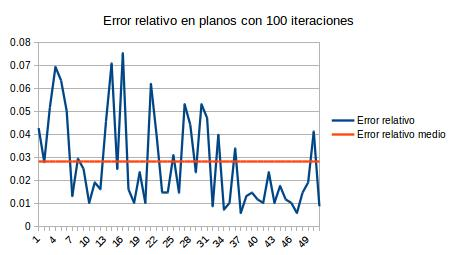
\includegraphics[width=8.5cm, height=5.0cm]{resultados/100_errRel.jpg}	
		\end{subfigure}%
		\begin{subfigure}[h]{.5\textwidth}
		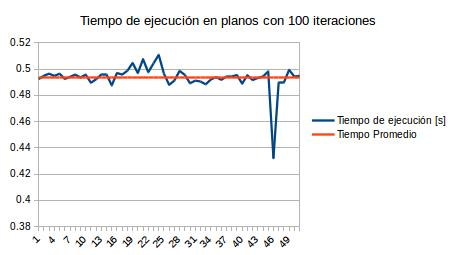
\includegraphics[width=8.5cm, height=5.0cm]{resultados/100_timeExec.jpg}
		\end{subfigure}
	
	\caption{Gráficas correspondientes al error relativo y tiempo de ejecución para el algoritmo RANSAC con 100 iteraciones.}

	\end{figure}

	\begin{figure}[H]

		\begin{subfigure}[h]{.5\textwidth}
		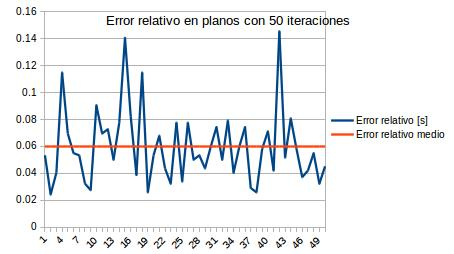
\includegraphics[width=8.5cm, height=5.0cm]{resultados/50_errRel.jpg}	
		\end{subfigure}%
		\begin{subfigure}[h]{.5\textwidth}
		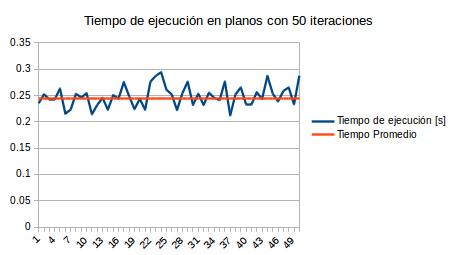
\includegraphics[width=8.5cm, height=5.0cm]{resultados/50_timeExec.jpg}
		\end{subfigure}
	
	\caption{Gráficas correspondientes al error relativo y tiempo de ejecución para el algoritmo RANSAC con 50 iteraciones.}

	\end{figure}

	\begin{figure}[H]

		\begin{subfigure}[h]{.5\textwidth}
		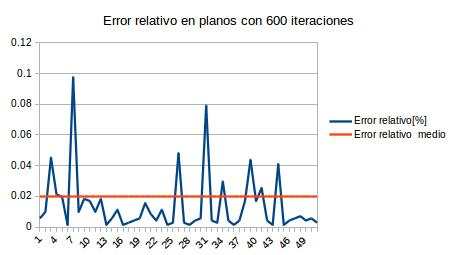
\includegraphics[width=8.5cm, height=5.0cm]{resultados/600_errRel.jpg}	
		\end{subfigure}%
		\begin{subfigure}[h]{.5\textwidth}
		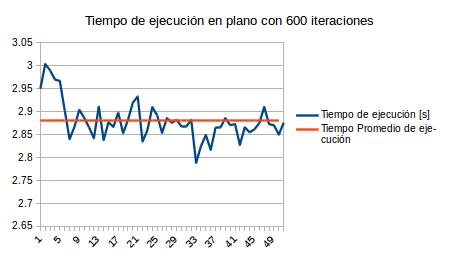
\includegraphics[width=8.5cm, height=5.0cm]{resultados/600_timeExec.jpg}
		\end{subfigure}
	
	\caption{Gráficas correspondientes al error relativo y tiempo de ejecución para el algoritmo RANSAC con 600 iteraciones.}

	\end{figure}

	\begin{figure}[ht!]

		\begin{subfigure}[h]{.5\textwidth}
		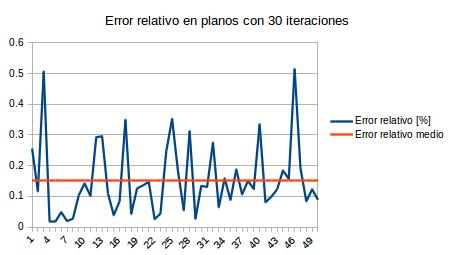
\includegraphics[width=8.5cm, height=5.0cm]{resultados/30_errRel.jpg}	
		\end{subfigure}%
		\begin{subfigure}[h]{.5\textwidth}
		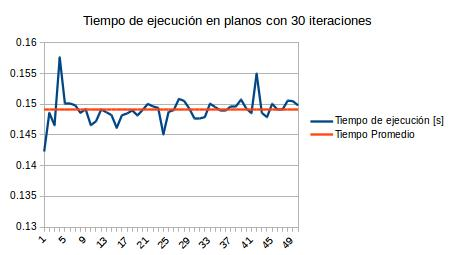
\includegraphics[width=8.5cm, height=5.0cm]{resultados/30_timeExec.jpg}
		\end{subfigure}
	
	\caption{Gráficas correspondientes al error relativo y tiempo de ejecución para el algoritmo RANSAC con 30 iteraciones.}

	\end{figure}

	\begin{figure}[H]

		\begin{subfigure}[h]{.5\textwidth}
		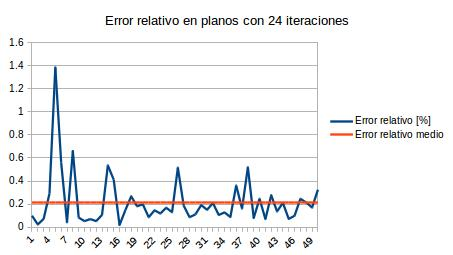
\includegraphics[width=8.5cm, height=5.0cm]{resultados/24_errRel.jpg}	
		\end{subfigure}%
		\begin{subfigure}[h]{.5\textwidth}
		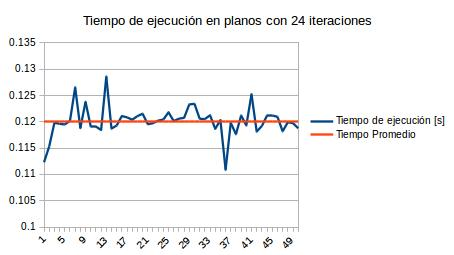
\includegraphics[width=8.5cm, height=5.0cm]{resultados/24_timeExec.jpg}
		\end{subfigure}
	
	\caption{Gráficas correspondientes al error relativo y tiempo de ejecución para el algoritmo RANSAC con 24 iteraciones.}

	\end{figure}

	\begin{figure}[H]

		\begin{subfigure}[h]{.5\textwidth}
		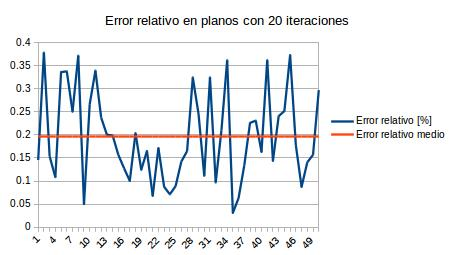
\includegraphics[width=8.5cm, height=5.0cm]{resultados/20_errRel.jpg}	
		\end{subfigure}%
		\begin{subfigure}[h]{.5\textwidth}
		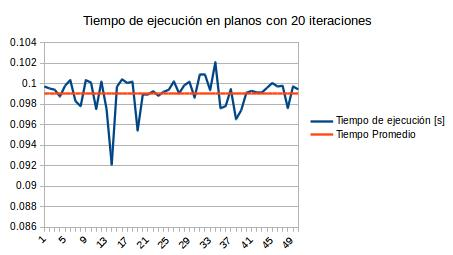
\includegraphics[width=8.5cm, height=5.0cm]{resultados/20_timeExec.jpg}
		\end{subfigure}
	
	\caption{Gráficas correspondientes al error relativo y tiempo de ejecución para el algoritmo RANSAC con 20 iteraciones.}

	\end{figure}

	Una vez que se obtuvo la información parcial de cada uno de estos eventos se realizó una tabla extra que agrupa la información del tiempo de ejecución promedio y el error relativo promedio contra el número de iteraciones del algoritmo. Se obtuvo la siguiente gráfica.\\

	\begin{figure}[H]

		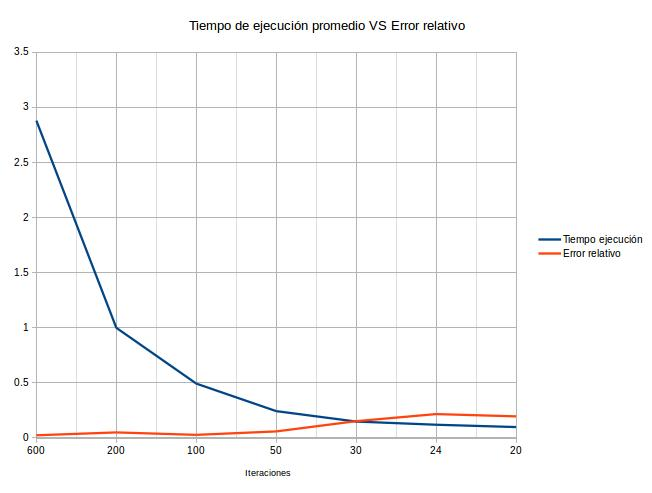
\includegraphics[width=14.5cm, height=8.0cm]{resultados/timeExec_errRel.jpg}
		\caption{Gráfica error relativo versus tiempo de ejecución para diferentes numeros de iteraciones.}

	\end{figure}


	Como podemos observar en la tabla 4.10 el error relativo presenta un incremento conforme se disminuye el número de iteraciones en el algoritmo. El tiempo de ejecución por su parte muestra un decremento conforme el número de iteraciones disminuye. Dado este comportamiento de ambos parámetros resulta difícil encontrar un punto de equilibrio entre estas dos unidades de medición. Sin embargo observamos que tanto el error relativo como el tiempo de ejecución llegan a un valor estable, a partir del cual no aumentan o disminuyen significativamente. La gráfica 4.10 nos sugiere que este punto está en un número de iteraciones entre 30 y 24.\\ 

	Por otro lado, se procedió a caracterizar la extracción de objetos y el cálculo de su centroide. Para ello se realizaron un total de 5 eventos con objetos diferentes, 1 prisma octagonal y 4 objetos comunes con formas regulares: prismas rectangules y cilindros. En cada uno de estos eventos se cálculo el centroide del objeto 130 veces, se tomaron medida de tendencia central (valor esperado del dentroide) y medidas de dispersión (varianza y desviación estándar). A continuación se presentan los resultados obtenidos de las mediciones realizadas.\\

	\begin{figure}[H]

		\begin{subfigure}[h]{.5\textwidth}
		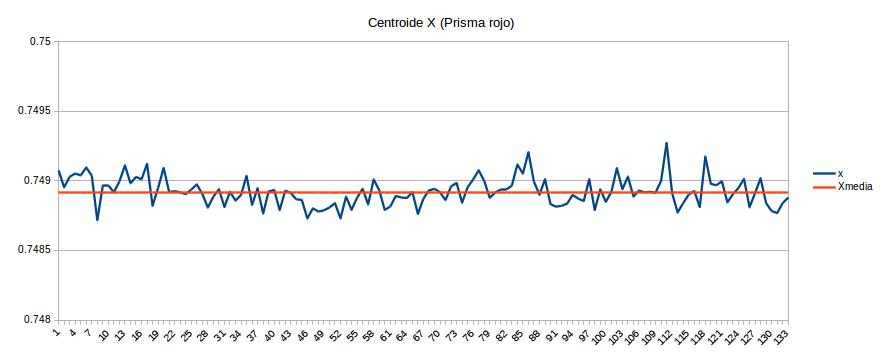
\includegraphics[width=14.5cm, height=6.0cm]{resultados/x_pRojo.jpg}	
		\end{subfigure}\\
		\begin{subfigure}[h]{.5\textwidth}
		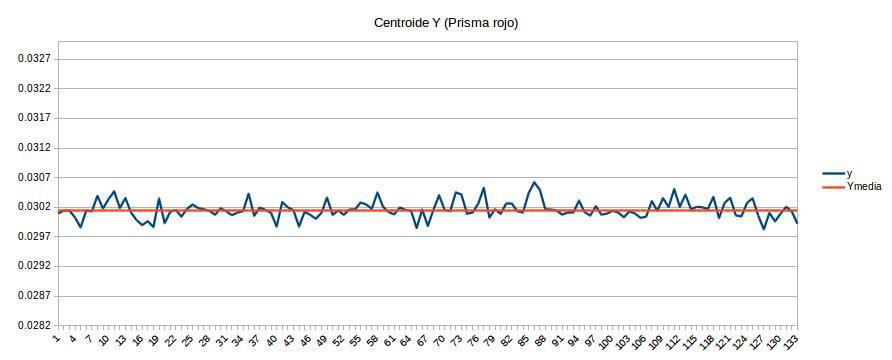
\includegraphics[width=14.5cm, height=6.0cm]{resultados/y_pRojo.jpg}
		\end{subfigure}\\
		\begin{subfigure}[h]{.5\textwidth}
		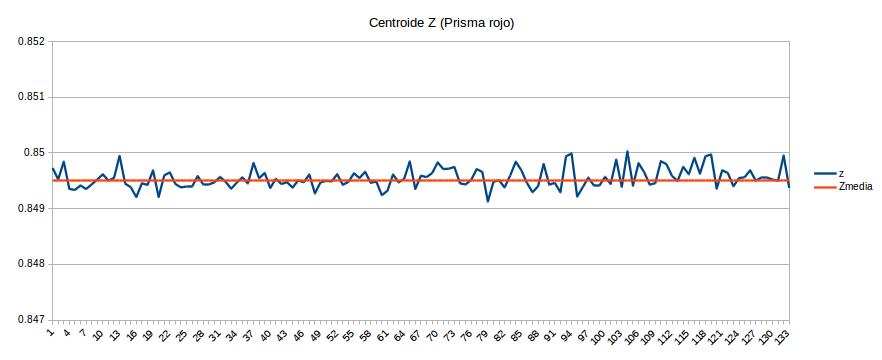
\includegraphics[width=14.5cm, height=6.0cm]{resultados/z_pRojo.jpg}
		\end{subfigure}
	
	\caption{Gráficas de coordenadas en centroide de un prisma rojo.}

	\end{figure}

	\begin{figure}[H]

		\begin{subfigure}[h]{.5\textwidth}
		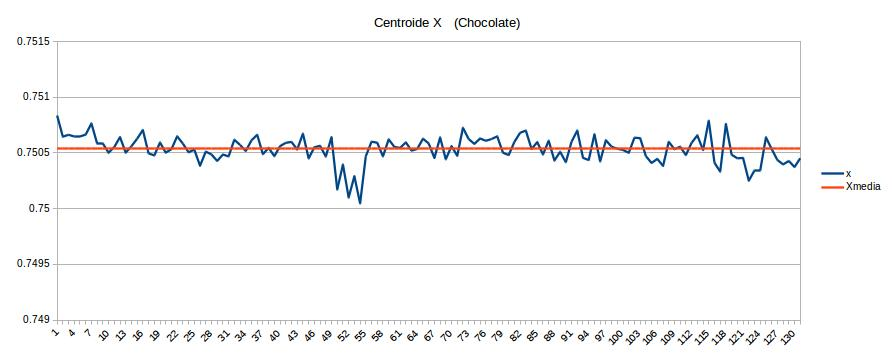
\includegraphics[width=14.5cm, height=6.0cm]{resultados/x_chocolate.jpg}	
		\end{subfigure}\\
		\begin{subfigure}[h]{.5\textwidth}
		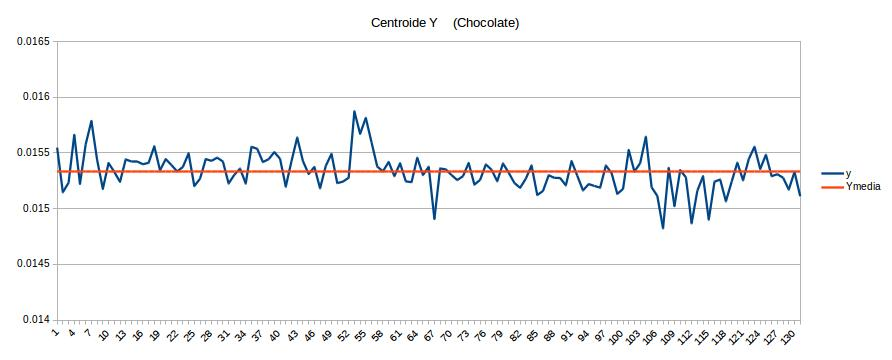
\includegraphics[width=14.5cm, height=6.0cm]{resultados/y_chocolate.jpg}
		\end{subfigure}\\
		\begin{subfigure}[h]{.5\textwidth}
		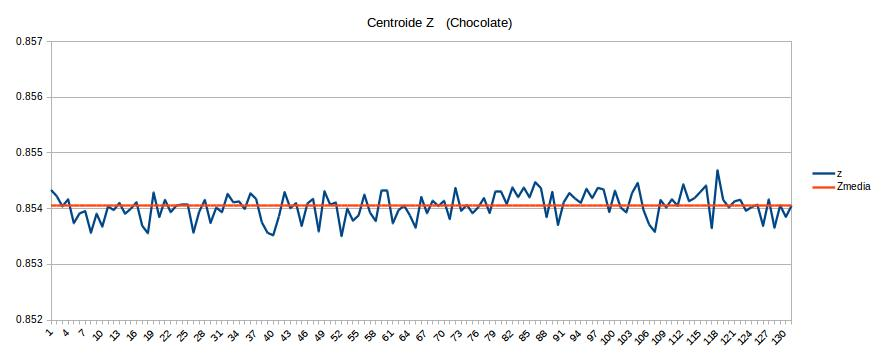
\includegraphics[width=14.5cm, height=6.0cm]{resultados/z_chocolate.jpg}
		\end{subfigure}
	
	\caption{Gráficas de coordenadas en centroide de una barra de chocolate.}

	\end{figure}

	\begin{figure}[H]

		\begin{subfigure}[h]{.5\textwidth}
		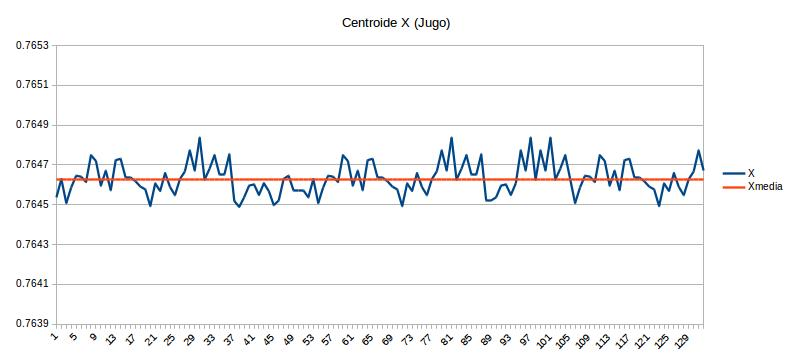
\includegraphics[width=14.5cm, height=6.0cm]{resultados/x_jugo.jpg}	
		\end{subfigure}\\
		\begin{subfigure}[h]{.5\textwidth}
		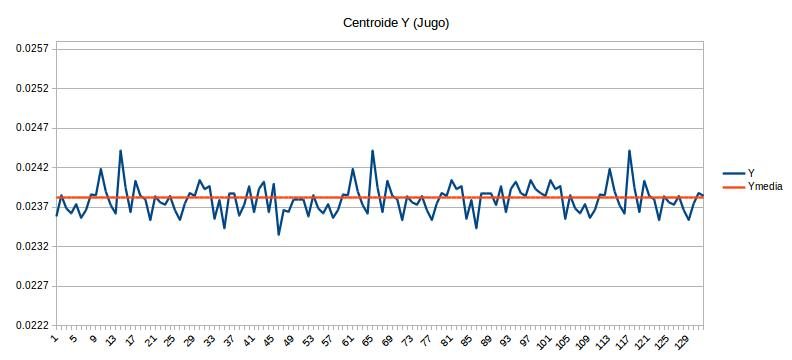
\includegraphics[width=14.5cm, height=6.0cm]{resultados/y_jugo.jpg}
		\end{subfigure}\\
		\begin{subfigure}[h]{.5\textwidth}
		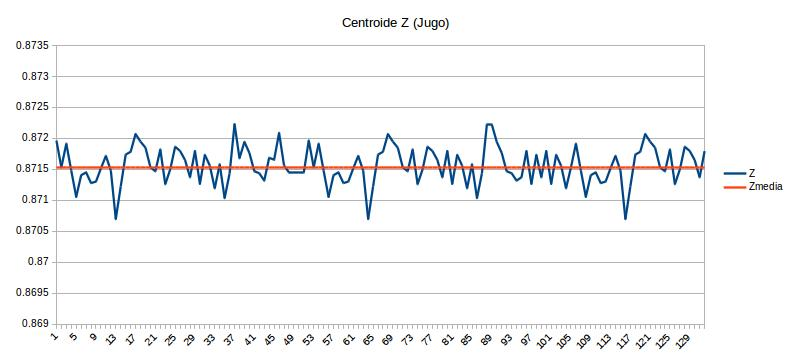
\includegraphics[width=14.5cm, height=6.0cm]{resultados/z_jugo.jpg}
		\end{subfigure}
	
	\caption{Gráficas de coordenadas en centroide de cartón de jugo.}

	\end{figure}

	\begin{figure}[H]

		\begin{subfigure}[h]{.5\textwidth}
		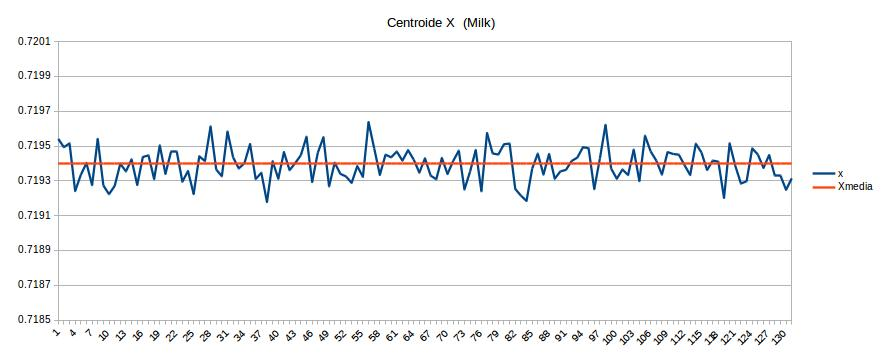
\includegraphics[width=14.5cm, height=6.0cm]{resultados/x_milk.jpg}	
		\end{subfigure}\\
		\begin{subfigure}[h]{.5\textwidth}
		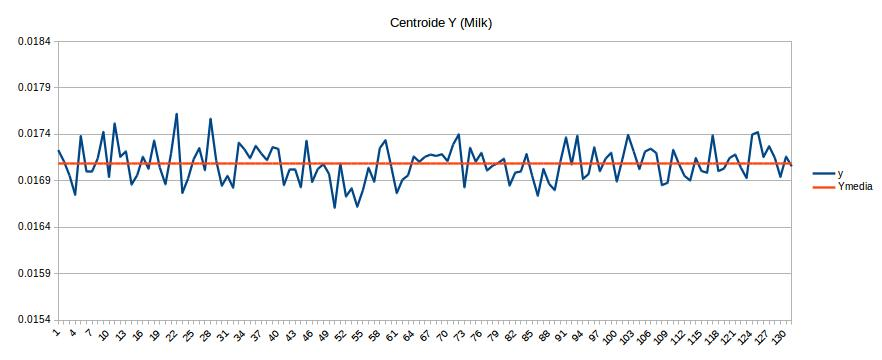
\includegraphics[width=14.5cm, height=6.0cm]{resultados/y_milk.jpg}
		\end{subfigure}\\
		\begin{subfigure}[h]{.5\textwidth}
		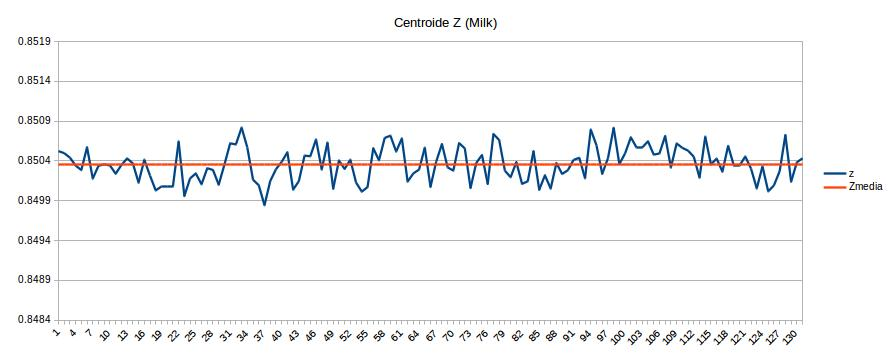
\includegraphics[width=14.5cm, height=6.0cm]{resultados/z_milk.jpg}
		\end{subfigure}
	
	\caption{Gráficas de coordenadas en centroide de un envase de leche.}

	\end{figure}

	\begin{figure}[H]

		\begin{subfigure}[h]{.5\textwidth}
		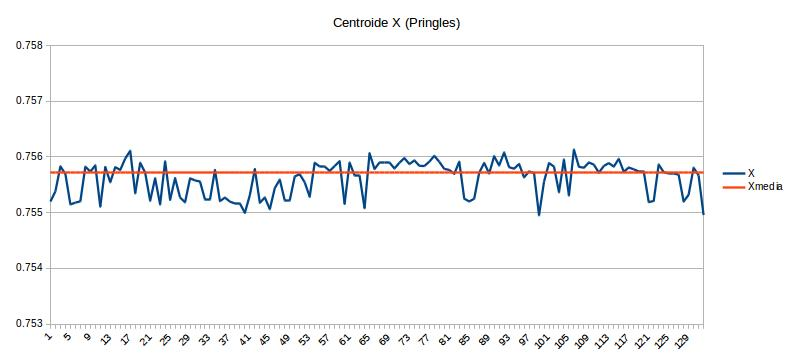
\includegraphics[width=14.5cm, height=6.0cm]{resultados/x_pringles.jpg}	
		\end{subfigure}\\
		\begin{subfigure}[h]{.5\textwidth}
		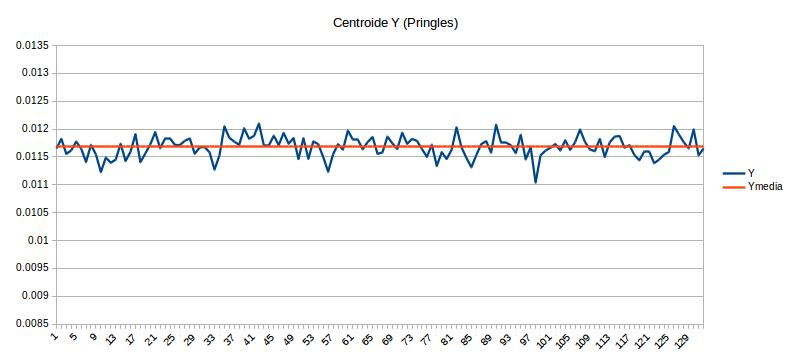
\includegraphics[width=14.5cm, height=6.0cm]{resultados/y_pringles.jpg}
		\end{subfigure}\\
		\begin{subfigure}[h]{.5\textwidth}
		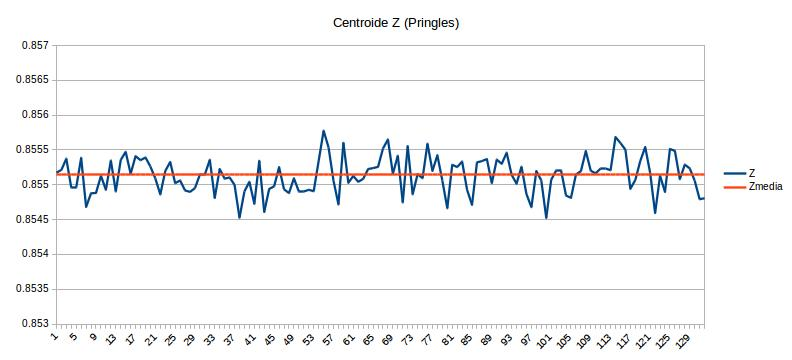
\includegraphics[width=14.5cm, height=6.0cm]{resultados/z_pringles.jpg}
		\end{subfigure}
	
	\caption{Gráficas de coordenadas en centroide de un contenedor de frituras (pringles).}

	\end{figure}

	La desviación estándar puede ser interpretada como una medida de incertidumbre. La desviación estándar de un grupo repetido de medidas nos da la precisión de éstas. Cuando se va a determinar si un grupo de medidas está de acuerdo con el modelo teórico, la desviación estándar de esas medidas es de vital importancia: si la media de las medidas está demasiado alejada de la predicción (con la distancia medida en desviaciones estándar), entonces consideramos que las medidas contradicen la teoría. Esto es coherente, ya que las mediciones caen fuera del rango de valores en el cual sería razonable esperar que ocurrieran si el modelo teórico fuera correcto. La desviación estándar es uno de tres parámetros de ubicación central; muestra la agrupación de los datos alrededor de un valor central (la media o promedio).\\

	\begin{figure}[H]
		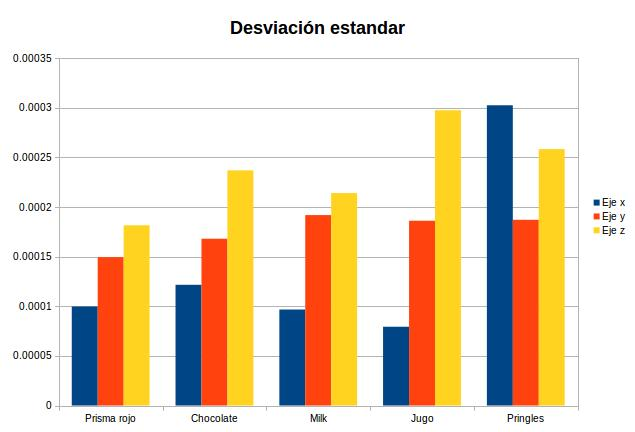
\includegraphics[width=14.5cm, height=7.0cm]{resultados/DesviacionEstandar.jpg}	
		\caption{Gráficas de desviciones estandar para diferentes objetos dispuestas por sus respectivos ejes.}
	\end{figure}




%%%%%%%%%%%%%%%%%%%%%%%%%%%%%%%%%%%%%%%%%%%%%%%%%%%%%%%%%%%%
%%%%%%%%%		Conclusiones           %%%%%%%%%%%%%%%%%%%%%
%% \chapter{Conclusiones} 
	Partiendo de la información obtenida de los resultados podemos concluir que un algoritmo RANSAC con un umbral de 0.5 [cm] y un número de iteraciones entre 24 y 30 nos ayudará a encontrar la ecuación de un plano así como una lista de puntos pertenecientes al mismo. Esta primera parte del desarrollo permitió desarrollar un algoritmo que no presentara un tiempo excesivo de ejecución de manera innecesaria. \\

	Una vez que se estuvo seguros que el algoritmo RANSAC funcionaba de manera aceptable se continuó a probar la extracción de objetos sobre el plano.\\

	Para ello se tomaron 5 muestras de objetos diferentes. Se calculó la media de las coordenadas \textit{x, y, z} y la desviación estándar de las mismas. En la Figura 4.15 podemos observar que el objeto que presentá una desviación estándar de mayor magnitud es el objeto \textit{pringles}, y de los tres ejes presenta una mayor desviación estándar en el eje $"z"$. El orden de magnitud de la mayor desviación estándar es de 0.3 milésimas. Entonces, por el concepto de la desviación estándar podemos decir que el cálculo de la media de los centroides del objetos tiene un alto grado de cercanía a la predicción (media) del mismo. Por tanto el cálculo de la media en cualquier instante es confiable.\\ 

